\documentclass{article}

\usepackage[a4paper]{geometry}
\usepackage[ngerman]{babel}
\usepackage[utf8]{inputenc}
\usepackage[T1]{fontenc}
\usepackage{tabularx}
\usepackage{graphicx}
\usepackage{fancyhdr}
\usepackage{pdflscape}

\graphicspath{ {./images/} }

\pagestyle{fancyplain}
\fancyhf{}
\lhead{\fancyplain{}{Maximilian Schulke} }
\rhead{\fancyplain{}{\today}}
\cfoot{\fancyplain{}{\thepage}}

\begin{document}

\begin{titlepage}
	\begin{flushleft}
		TH Brandenburg \\
		Online Studiengang Medieninformatik \\
		Fachbereich Informatik und Medien \\
		Mensch-Computer-Interaktion \\
		Prof. Dr. Martin Christof Kindsmüller
	\end{flushleft}

	\vfill

	\begin{center}
		\Large{Einsendeaufgabe 1: Personas und Storyboards}\\[0.5em]
		\large{Sommersemester 2021}\\[0.25em]
		\large{Abgabetermin 01.05.2021}
	\end{center}

	\vfill

	\begin{flushright}
		Maximilian Schulke \\
		Matrikel-Nr. 20215853
	\end{flushright}
\end{titlepage}

\tableofcontents

\vfill

\section{Aufgabenstellung}

Folgende Aufgabenstellung wurde im Moodle-Kurs bekannt gegeben:

\begin{quote}
	Sie haben die Aufgabe eine Smartphone-App zu konzipieren, die OSMI-Studierende beim Studium unterstützt.
	Die App soll insbesondere die Kommunikation, die gegenseitige Unterstützung und das gemeinsame Bearbeiten
	von Aufgaben und Projekten unterstützen. Denken Sie auch darüber nach, wie die App in der aktuellen
	SARS-CoV-2-Situation helfen kann (also beispielsweise auch Studierende, die normalerweise in Präsenz studieren).
	\\[1em]
	(a) Erstellen Sie zwei Personas der (potentiellen) Zielgruppe.

	(b) Erstellen Sie für jede Persona zwei Storyboards (also insgesamt vier) zur Nutzung der App. Storyboards
	werden in der Regel von Hand gezeichnet (auf Schönheit kommt es in diesem Zusammenhang nicht an). Scannen
	oder fotografieren Sie die Skizzen und beschreiben Sie ggf. kurz wie die Skizzen verstanden werden sollen.
	\\[1em]
	Anmerkungen:

	Abzugeben ist ein PDF-Dokument, das Ihre Ausführungen enthält. Bitte beachten Sie dazu die Hinweise zu den
	Einsendeaufgaben (siehe oben). Der zeitliche Umfang dieser Einsendeaufgabe wird auf 6 Stunden geschätzt.
	Ihre Ausarbeitung sollte ca. 7-9 Seiten (A4) umfassen (eine Seite für Titelblatt inkl. Aufgabenstellung,
	je eine Seite pro Persona, und je eine pro Storyboard sowie ggf. zusätzliche Seiten für die Erläuterungen).
	Die Lösung, die Sie zur Deadline abgeben, sollte eine aus Ihrer Sicht endgültige Lösung sein. Falls Sie
	Fragen zur Aufgabenstellung haben, stellen Sie diese bitte im Vorfeld!
\end{quote}

\newpage

\section{Personas}

\subsection{Mark Schneider - Der Effiziente}

\begin{figure}[h]
	
\includegraphics[width=0.25\textwidth]{mark}
	\centering
	\caption{Mark Schneider – thispersondoesnotexist.com}
\end{figure}

\vspace{-1em}

\begin{quote}
	``Ich verbringe meine Zeit gerne mit meiner Familie. Wenn ich Abends noch studiere, dann versuche
	ich möglichst effizient durch den Stoff zu kommen. Bisher habe ich eher selten in Lerngruppen gearbeitet,
	da mir der Austausch mit anderen Studenten immer sehr Zeitaufwendig vorkam.`` - Mark
\end{quote}

\vspace{0em}

\begin{flushleft}
	\textbf{Verhaltensweisen} \\
	Überspringt meistens die Skripte und versucht direkt die Aufgaben zu bearbeiten um schnell durchzukommen.
	Lernt gerne durch Videos, und schaut diese auf 1.5-facher Geschwindigkeit. Versucht mit so wenig Einsatz
	wie möglich durch die Klausur zu kommen.\\
	\vspace{1em}

	\textbf{Motivation für OSMI} \\
	Möchte einen Karrieresprung machen, um mehr Geld für seine Familie zu verdienen - er bekam Kontakt zum
	OSMI als Weiterbildungsprogramm in seinem Job an einer Hochschule. \\

	\vspace{1em}

	\textbf{Motivation für Lerngruppen} \\
	Mark hat durch seine relativ begrenzten Zeiteinsatz öfter Probleme und ist dankbar wenn er unkompliziert mit
	anderen seine Probleme besprechen und lösen kann.
\end{flushleft}

\vspace{1em}

\begin{center}
	\begin{tabularx}{\textwidth}{|l|X|}
		\hline
		\textbf{Eckdaten}  &                                     \\
		\hline
		Name               & Marc Schneider                      \\
		\hline
		Alter              & 28                                  \\
		\hline
		Beruf              & Hochschul-Verwaltungsangestellter   \\
		\hline
		Bildungsabschluss  & Abitur                              \\
		\hline
		Familienstand      & Verheiratet                         \\
		\hline
		Kinder             & Ja                                  \\
		\hline
		Wohnort            & Brandenburg an der Havel            \\
		\hline
		Hobbies            & Alte Filme sammeln, Kochen, Wandern \\
		\hline
		OSMI-Student seit  & WS 2019                             \\
		\hline
		Persönlichkeitstyp & Introvertiert                       \\
		\hline
	\end{tabularx}
\end{center}

\newpage

\subsection{Rosa Haas - Die Motivierte}

\begin{figure}[h]
	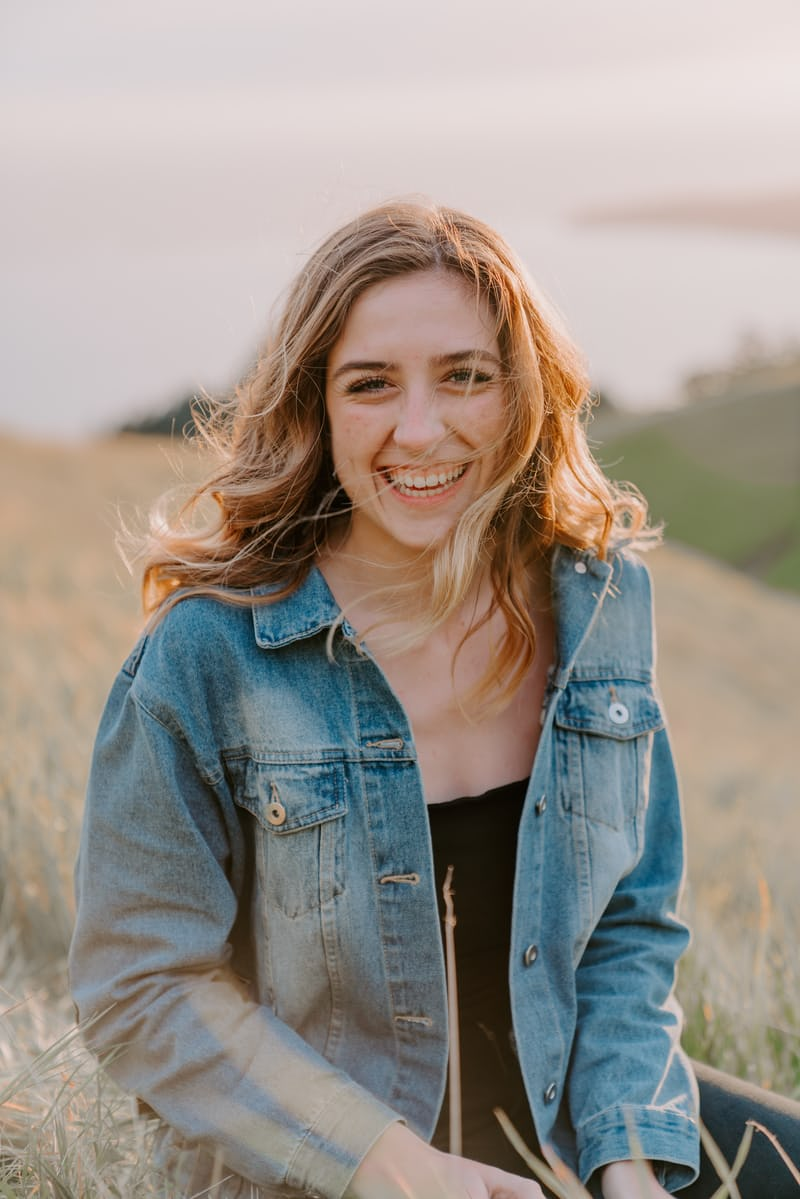
\includegraphics[width=0.25\textwidth]{rosa}
	\centering
	\caption{Rosa Haas – thispersondoesnotexist.com}
\end{figure}

\begin{quote}
	``Ich bin gerne mit anderen Menschen zusammen und finde, dass das Studium
	zusammen viel mehr Spaß macht und man besser lernt. Deshalb habe ich mit einigen
	Kommilitonen eine Lerngruppe gegründet.`` - Rosa
\end{quote}

\vspace{0em}

\begin{flushleft}
	\textbf{Verhaltensweisen} \\
	Fängt bereits sehr früh an für Klausuren zu lernen, da sie gerne die Situation unter Kontrolle hat.
	Ist sehr interessiert an Informatik und schaut auch gerne über den Modulinhalt hinaus.
	\vspace{1em}

	\textbf{Motivation für OSMI} \\
	Möchte sich in Richtung Informatik weiterentwickeln und sich selbst etwas Beweisen. Möchte letztendlich
	auch mehr Geld durch das Studium verdienen, aber die neugier war ausschalggebend für die Enschreibung. \\
	\vspace{1em}

	\textbf{Motivation für Lerngruppen} \\
	Rosa trifft sich gerne mit anderen zum lernen und tauscht sich gerne über den Stoff aus, da sie den
	Kontakt zu anderen beim Online-Studiunm etwas vermisst.
\end{flushleft}

\vspace{1em}

\begin{center}
	\begin{tabularx}{\textwidth}{|l|X|}
		\hline
		\textbf{Eckdaten}  &                                              \\
		\hline
		Name               & Rosa Haas                                    \\
		\hline
		Alter              & 23                                           \\
		\hline
		Beruf              & Screen Desginerin                            \\
		\hline
		Bildungsabschluss  & Ausbildung                                   \\
		\hline
		Familienstand      & Ledig                                        \\
		\hline
		Kinder             & Nein                                         \\
		\hline
		Wohnort            & Berlin Wedding                               \\
		\hline
		Hobbies            & Netflix, Feiern, guter Kaffee \& Kreativität \\
		\hline
		OSMI-Student seit  & SS 2021                                      \\
		\hline
		Persönlichkeitstyp & Extrovertiert                                \\
		\hline
	\end{tabularx}
\end{center}

\newpage

\begin{landscape}
	\section{Storyboards}

	\subsection{Storyboard 1 für Mark}

	\begin{figure}[h!]
		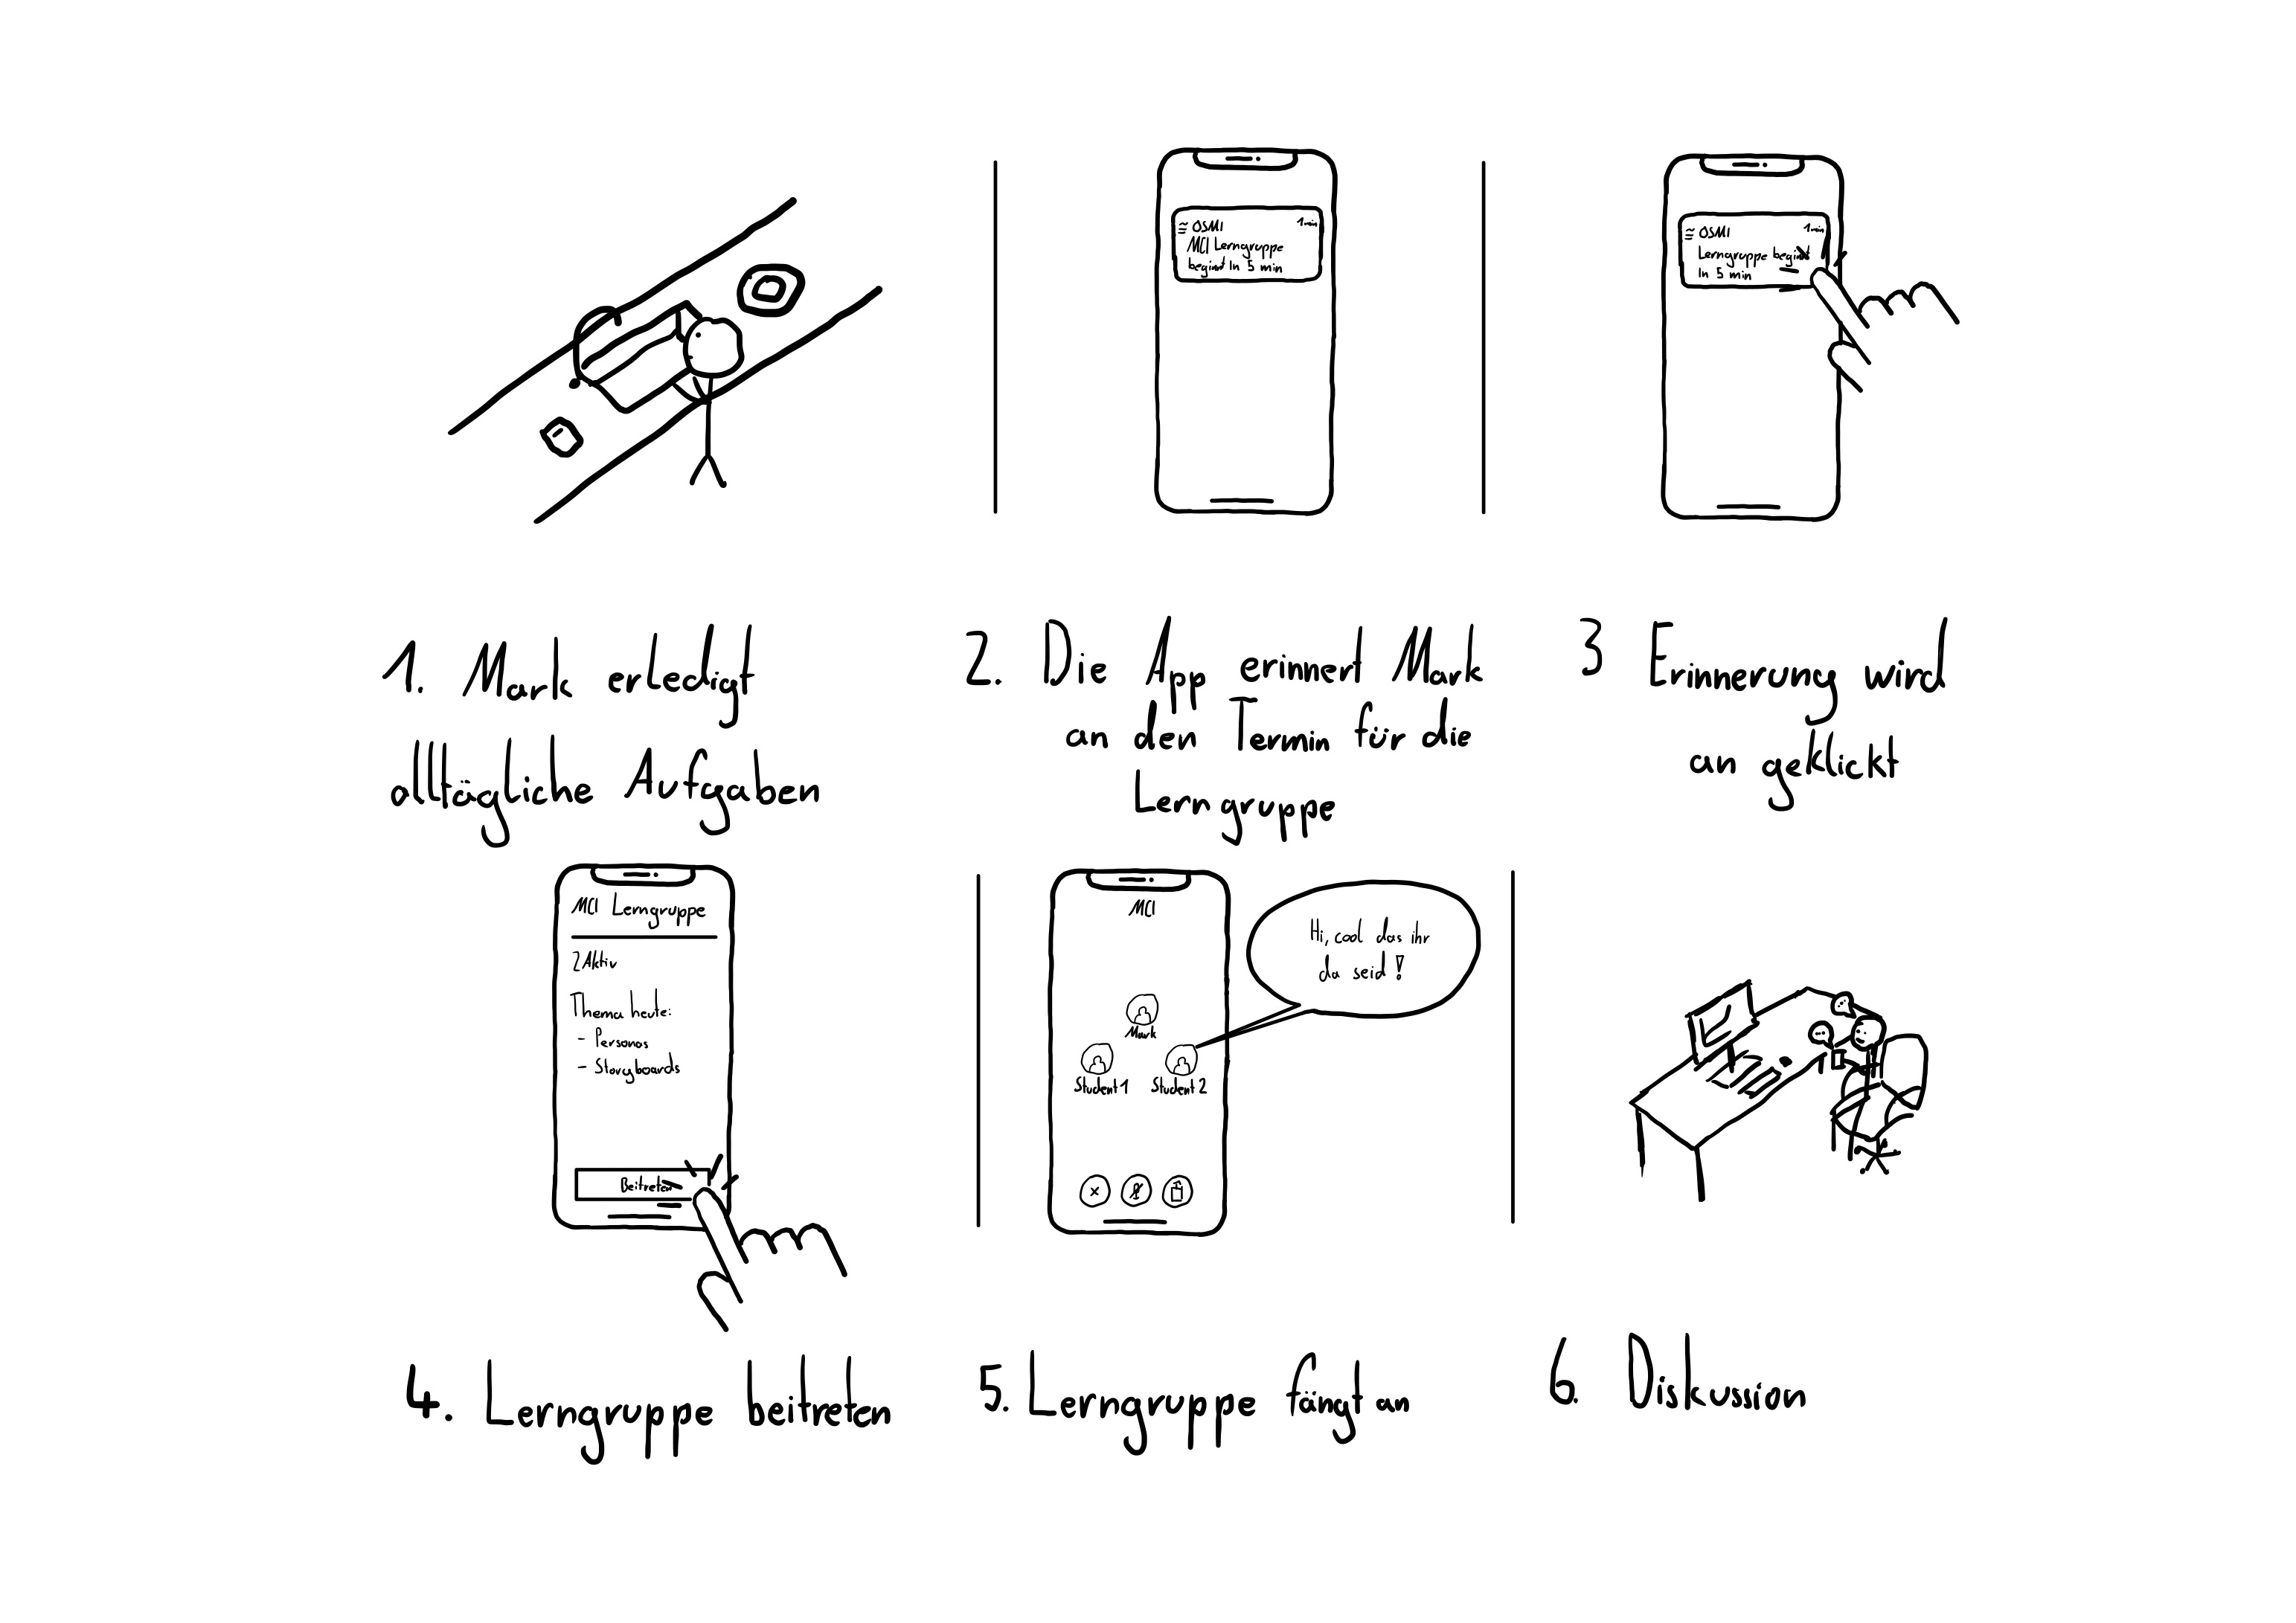
\includegraphics[height=0.7\textheight]{storyboard-1-mark}
		\centering
		\caption{Storyboard Mark – Als OSMI Student möchte ich über Lerngruppen-Termine benachrichtigt werden, da ich diese sonst u.U. verpasse.}
	\end{figure}

	\newpage

	\subsection{Storyboard 2 für Mark}

	\begin{figure}[h!]
		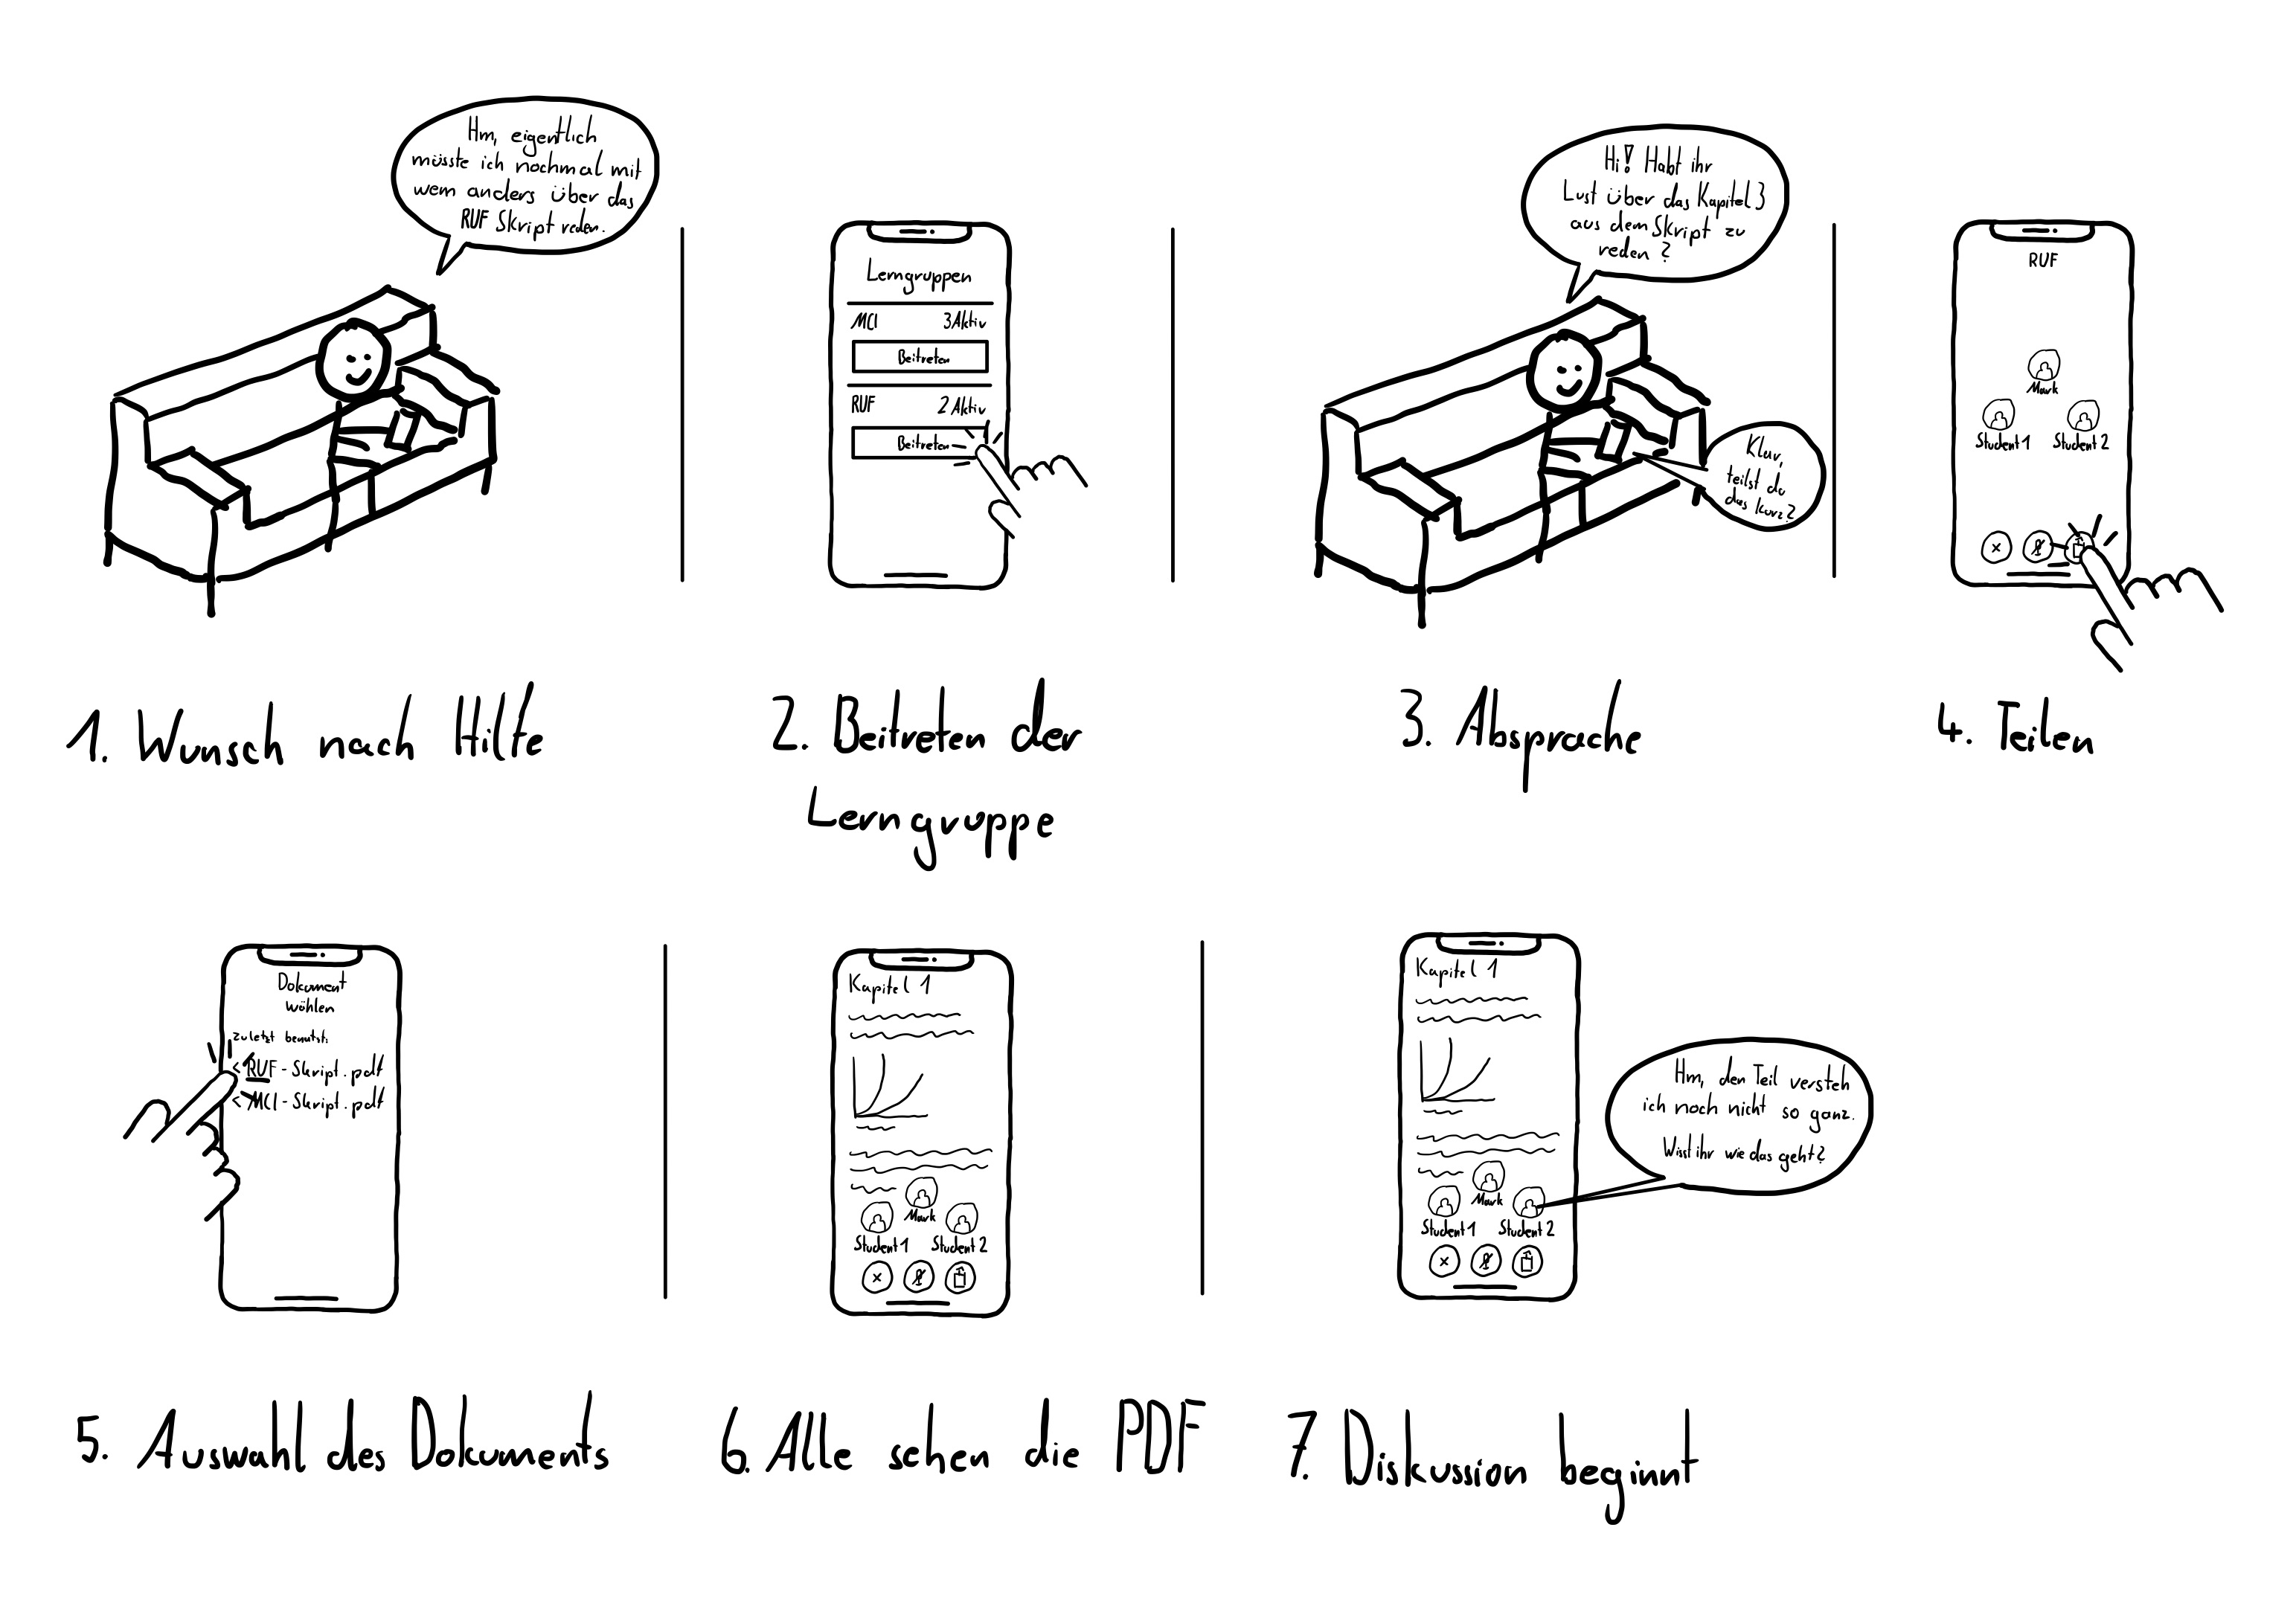
\includegraphics[height=0.7\textheight]{storyboard-2-mark}
		\centering
		\caption{Storyboard Mark – Als OSMI Student möchte ich unkompliziert mit anderen Studenten in einer PDF zusammenarbeiten, um den Zeitaufwand der Zusammenarbeit zu minimieren.}
	\end{figure}

	\newpage

	\subsection{Storyboard 3 für Rosa}

	\begin{figure}[h!]
		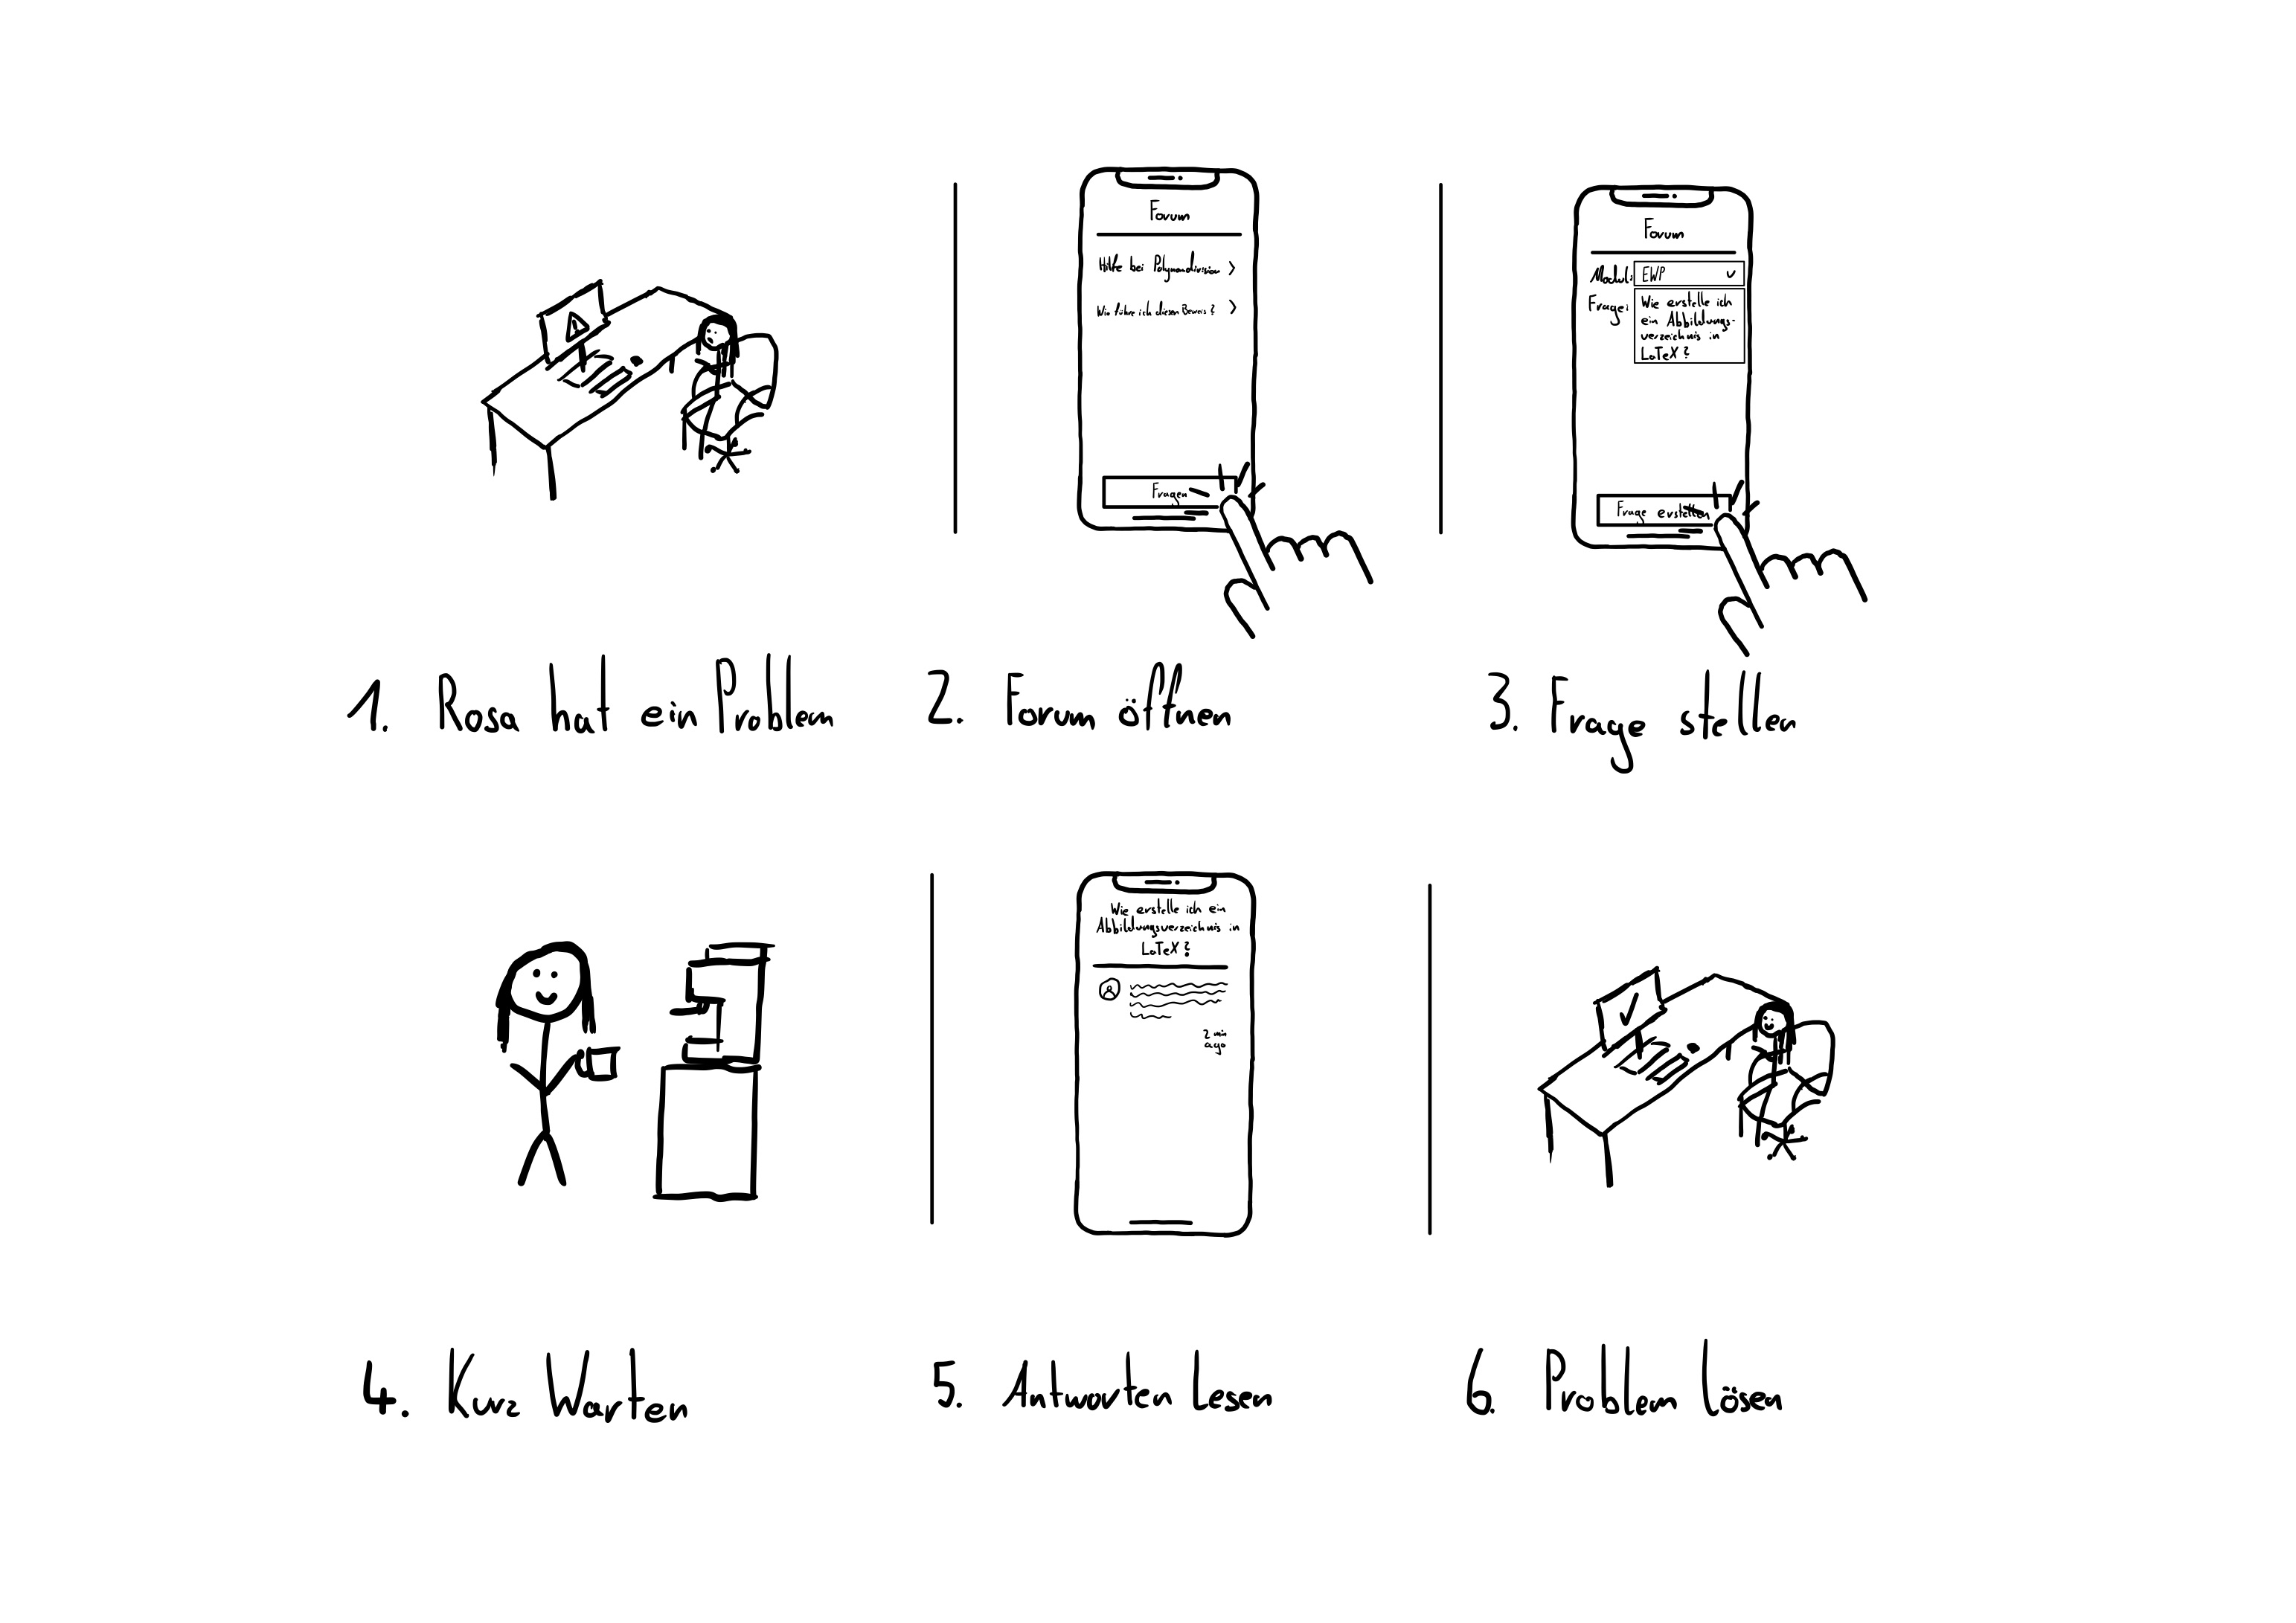
\includegraphics[height=0.7\textheight]{storyboard-3-rosa}
		\centering
		\caption{Storyboard Rosa – Als OSMI Student möchte ich Fragen in ein Forum posten, um bei Problemen schnell Hilfe von anderen Studenten zu bekommen.}
	\end{figure}

	\newpage

	\subsection{Storyboard 4 für Rosa}

	\begin{figure}[h!]
		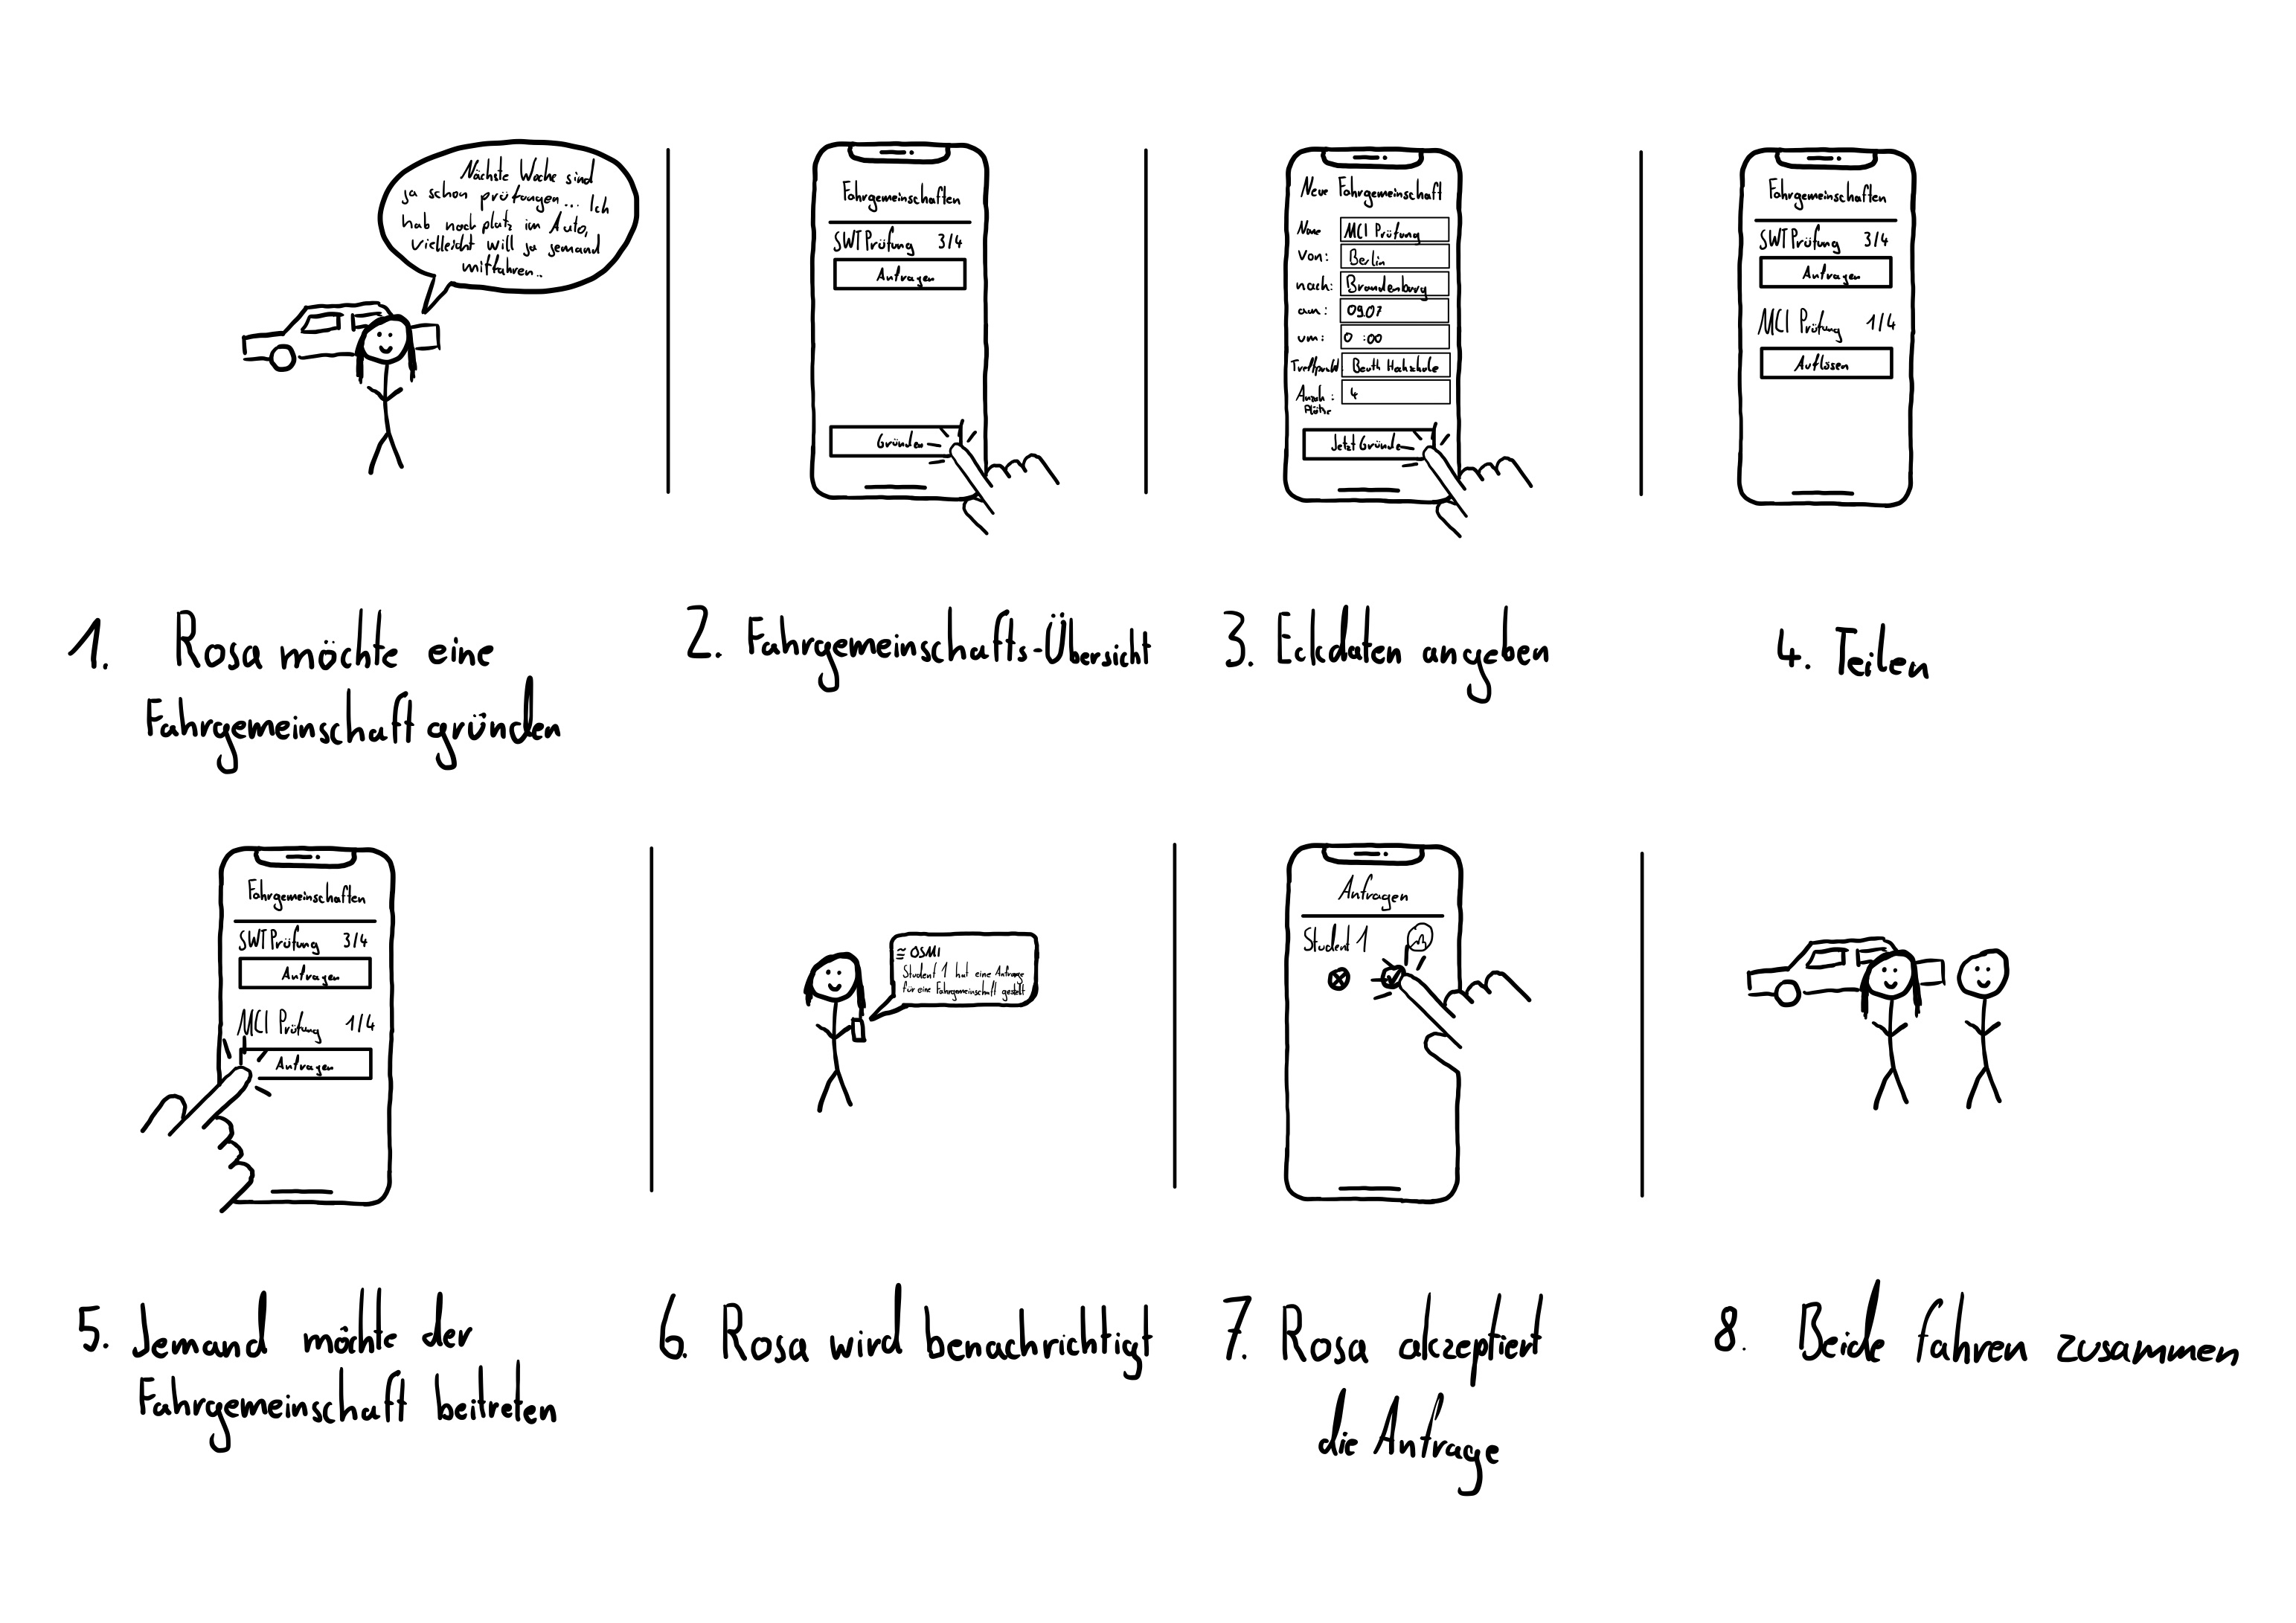
\includegraphics[height=0.7\textheight]{storyboard-4-rosa}
		\centering
		\caption{Storyboard Rosa – Als OSMI Student möchte ich Fahrgemeinschaften gründen, um mir Fahrtkosten zu sparen und die Umwelt zu schonen.}
	\end{figure}
\end{landscape}

\end{document}